\documentclass[conference]{IEEEtran}

\usepackage[utf8]{inputenc}
\usepackage{cite}
\usepackage{amsmath,amssymb,amsfonts}
\usepackage{graphicx}
\usepackage{xcolor}
\usepackage{tikz}
\usetikzlibrary{shapes.geometric, arrows.meta, positioning, fit, calc, backgrounds, patterns, circuits.logic.US, shapes.misc}
\usepackage{pgfplots}
\pgfplotsset{compat=1.17}
\usepackage{subcaption}
\usepackage{booktabs}

% Hardware component styles
\tikzset{
    register/.style={
        rectangle,
        draw=black,
        thick,
        minimum width=1.2cm,
        minimum height=0.8cm,
        fill=white,
        font=\scriptsize\ttfamily
    },
    mux/.style={
        trapezium,
        trapezium left angle=70,
        trapezium right angle=110,
        draw=black,
        thick,
        minimum width=0.8cm,
        minimum height=0.6cm,
        fill=white,
        font=\tiny
    },
    alu/.style={
        rectangle,
        draw=black,
        thick,
        minimum width=1cm,
        minimum height=1.2cm,
        fill=white,
        font=\scriptsize
    },
    memory/.style={
        rectangle,
        draw=black,
        very thick,
        minimum width=1cm,
        minimum height=1.5cm,
        fill=white,
        font=\scriptsize
    },
    wire/.style={
        draw=black,
        thick,
        -Stealth
    },
    bus/.style={
        draw=black,
        line width=1.5pt,
        -Stealth
    },
    controlwire/.style={
        draw=black,
        dashed,
        -Stealth
    },
    buswidth/.style={
        font=\tiny,
        fill=white,
        inner sep=1pt
    },
    dff/.style={
        rectangle,
        draw=black,
        thick,
        minimum width=0.6cm,
        minimum height=0.8cm,
        fill=white,
        font=\tiny
    },
    logic/.style={
        rectangle,
        draw=black,
        thick,
        rounded corners=2pt,
        minimum width=0.8cm,
        minimum height=0.6cm,
        fill=gray!10,
        font=\tiny
    },
    sbox/.style={
        rectangle,
        draw=black,
        thick,
        minimum width=0.7cm,
        minimum height=0.7cm,
        fill=gray!20,
        font=\tiny
    }
}

\begin{document}

\title{AES-128 Hardware Architecture:\\RTL Implementation on FPGA}

\author{\IEEEauthorblockN{Hardware Implementation}
\IEEEauthorblockA{Register-Transfer Level Design}}

\maketitle

%==============================================================================
% Figure 1: Complete Datapath Architecture
%==============================================================================
\begin{figure*}[t]
\centering
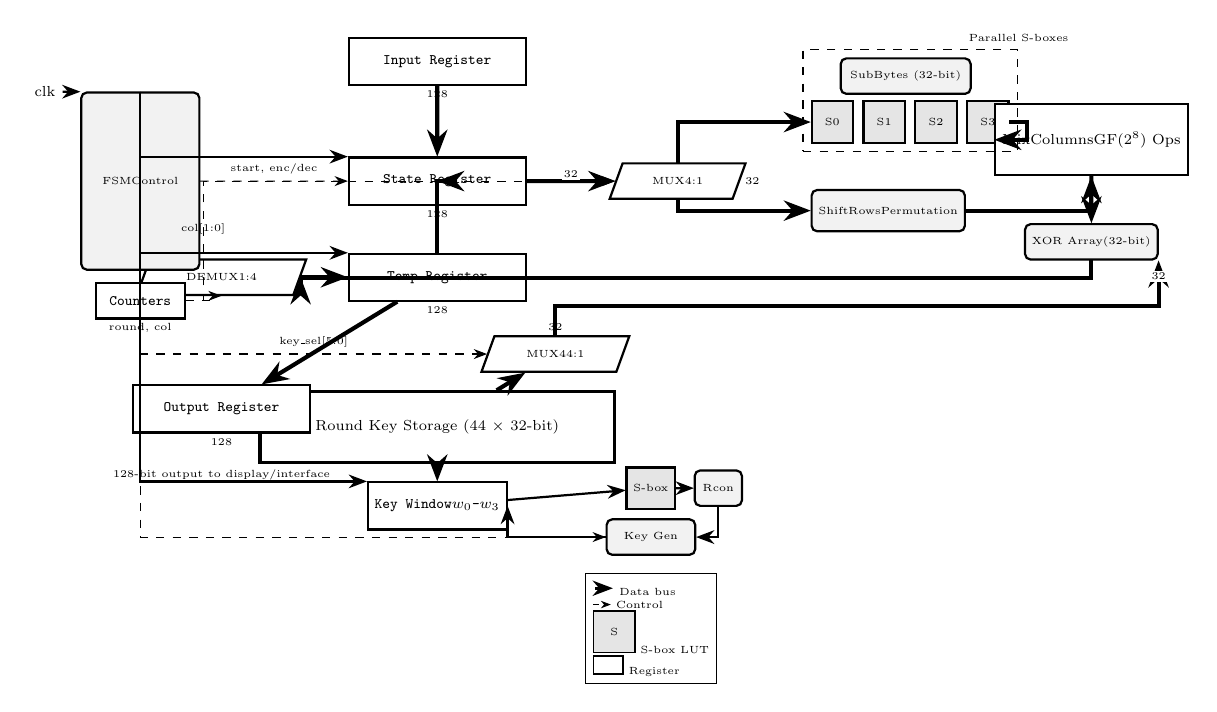
\begin{tikzpicture}[node distance=0.8cm and 1cm, scale=0.75, transform shape]

% Input Register
\node[register, minimum width=3cm] (input_reg) {Input Register};
\node[buswidth] at (input_reg.south) [below=0.05cm] {128};

% State Register (main storage)
\node[register, minimum width=3cm, below=1.2cm of input_reg] (state_reg) {State Register};
\node[buswidth] at (state_reg.south) [below=0.05cm] {128};

% Column Multiplexer
\node[mux, right=1.5cm of state_reg, minimum width=1.5cm] (col_mux) {MUX\\4:1};
\node[buswidth] at (col_mux.east) [right=0.05cm] {32};

% Datapath Components (32-bit wide)
\node[sbox, right=1.2cm of col_mux, yshift=1cm] (sbox0) {S0};
\node[sbox, right=0.15cm of sbox0] (sbox1) {S1};
\node[sbox, right=0.15cm of sbox1] (sbox2) {S2};
\node[sbox, right=0.15cm of sbox2] (sbox3) {S3};
\node[logic, above=0.1cm of sbox1.north east, minimum width=2.2cm] (subbytes_label) {SubBytes (32-bit)};

% ShiftRows Logic
\node[logic, right=1.2cm of col_mux, yshift=-0.5cm, minimum width=2cm, minimum height=0.7cm] (shiftrows) {ShiftRows\\Permutation};

% MixColumns (GF multipliers)
\node[alu, right=1.5cm of sbox1, yshift=-0.3cm, minimum width=1.8cm, minimum height=1.2cm] (mixcol) {MixColumns\\GF($2^8$) Ops};

% AddRoundKey (XOR array)
\node[logic, below=0.8cm of mixcol, minimum width=1.8cm] (xor_array) {XOR Array\\(32-bit)};

% Temporary Register
\node[register, below=0.8cm of state_reg, minimum width=3cm] (temp_reg) {Temp Register};
\node[buswidth] at (temp_reg.south) [below=0.05cm] {128};

% Column Demultiplexer
\node[mux, left=0.8cm of temp_reg, minimum width=1.5cm, shape border rotate=180] (col_demux) {DEMUX\\1:4};

% Key Expansion Unit (bottom)
\node[memory, below=1.5cm of temp_reg, minimum width=6cm, minimum height=1.2cm] (key_storage) {Round Key Storage (44 $\times$ 32-bit)};

\node[register, below=0.3cm of key_storage, minimum width=2cm] (key_window) {Key Window\\$w_0$-$w_3$};

\node[sbox, right=2cm of key_window, yshift=0.3cm] (key_sbox) {S-box};
\node[logic, right=0.3cm of key_sbox] (key_rcon) {Rcon};
\node[logic, below=0.15cm of key_sbox, minimum width=1.5cm] (key_gen) {Key Gen};

% Round Key Multiplexer
\node[mux, above=0.3cm of key_storage, minimum width=1.5cm, xshift=2cm] (rkey_mux) {MUX\\44:1};
\node[buswidth] at (rkey_mux.north) [above=0.05cm] {32};

% Output Register
\node[register, minimum width=3cm, below=1.5cm of col_demux] (output_reg) {Output Register};
\node[buswidth] at (output_reg.south) [below=0.05cm] {128};

% Control Signals
\node[logic, left=2.5cm of state_reg, minimum width=2cm, minimum height=3cm] (fsm) {FSM\\Control};
\node[register, below=0.2cm of fsm, minimum width=1.5cm, minimum height=0.6cm] (counters) {Counters};
\node[buswidth] at (counters.south) [below=0.02cm, font=\tiny] {round, col};

% Data Path Connections
\draw[bus] (input_reg) -- (state_reg);
\draw[bus] (state_reg) -- node[buswidth, above] {32} (col_mux);
\draw[bus] (col_mux.north) |- (sbox0.west);
\draw[bus] (sbox3.east) -- ++(0.3,0) |- (mixcol.west);
\draw[bus] (col_mux.south) |- (shiftrows.west);
\draw[bus] (shiftrows.east) -| (mixcol.south);
\draw[bus] (mixcol) -- (xor_array);
\draw[bus] (xor_array.south) -- ++(0,-0.3) -| (col_demux.east);
\draw[bus] (col_demux) -- (temp_reg);
\draw[bus] (temp_reg) |- (state_reg);
\draw[bus] (temp_reg) -- (output_reg);

% Key Path
\draw[bus] (key_storage) -- (rkey_mux);
\draw[bus] (rkey_mux.north) -- ++(0,0.5) -| node[buswidth, near end, above] {32} (xor_array.south east);
\draw[bus] (key_storage.south) -- (key_window);
\draw[wire] (key_window) -- (key_sbox);
\draw[wire] (key_sbox) -- (key_rcon);
\draw[wire] (key_rcon) |- (key_gen);
\draw[wire] (key_gen) -| (key_window.east);

% Control Signals
\draw[controlwire] (fsm.east) -- node[above, font=\tiny] {start, enc/dec} (state_reg.west);
\draw[controlwire] (counters.east) -- ++(0.3,0) |- node[near start, above, font=\tiny] {col[1:0]} (col_mux.west);
\draw[controlwire] (counters.east) -- ++(0.5,0) |- (col_demux.south);
\draw[controlwire] (fsm) |- node[near end, above, font=\tiny] {key\_sel[5:0]} (rkey_mux.west);
\draw[controlwire] (fsm) |- (key_gen.west);

% Clock
\node[left=0.3cm of fsm.north west] (clk_in) {\scriptsize clk};
\draw[wire] (clk_in) -- (fsm.north west);
\draw[wire] (fsm.north) |- (state_reg.north west);
\draw[wire] (fsm.north) |- (temp_reg.north west);
\draw[wire] (fsm.north) |- (key_window.north west);

% Annotations
\node[draw, dashed, fit=(sbox0) (sbox3) (subbytes_label), inner sep=0.1cm, label={[font=\tiny]above right:Parallel S-boxes}] {};
\node[font=\tiny, below=0.5cm of output_reg] {128-bit output to display/interface};

% Legend
\node[draw, rectangle, fill=white, below=0.3cm of key_gen, align=left, font=\tiny] {
\tikz{\draw[bus] (0,0) -- (0.3,0);} Data bus\\
\tikz{\draw[controlwire] (0,0) -- (0.3,0);} Control\\
\tikz{\node[sbox] {S};} S-box LUT\\
\tikz{\node[register, minimum width=0.5cm, minimum height=0.3cm] {};} Register
};

\end{tikzpicture}
\caption{Complete AES datapath architecture showing register-transfer level implementation. The design uses column-wise processing with a 32-bit datapath, four parallel S-boxes, and explicit register staging. Control signals manage column/round iteration and key selection.}
\label{fig:datapath_arch}
\end{figure*}

%==============================================================================
% Figure 2: AES Round Pipeline Structure
%==============================================================================
\begin{figure*}[t]
\centering
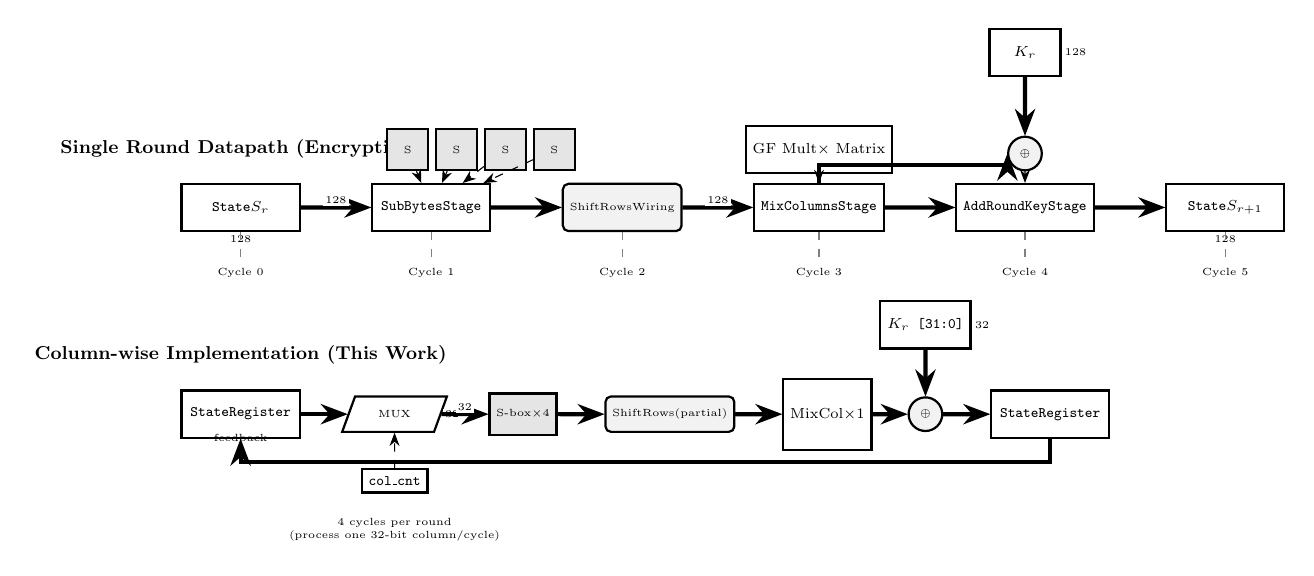
\begin{tikzpicture}[node distance=0.6cm and 1.2cm, scale=0.75, transform shape]

% Pipeline stages for one round
\node[font=\small\bfseries] at (0,3) {Single Round Datapath (Encryption)};

% Stage 1: State Input
\node[register, minimum width=2cm] (s0) at (0,2) {State\\$S_r$};
\node[buswidth] at (s0.south) [below=0.02cm] {128};

% Stage 2: SubBytes
\node[register, minimum width=2cm, right=of s0] (sb_reg) {SubBytes\\Stage};
\node[sbox, above=0.2cm of sb_reg, xshift=-0.4cm] (sb0) {S};
\node[sbox, right=0.1cm of sb0] (sb1) {S};
\node[sbox, right=0.1cm of sb1] (sb2) {S};
\node[sbox, right=0.1cm of sb2] (sb3) {S};
\draw[controlwire] (sb0) -- (sb_reg);
\draw[controlwire] (sb1) -- (sb_reg);
\draw[controlwire] (sb2) -- (sb_reg);
\draw[controlwire] (sb3) -- (sb_reg);

% Stage 3: ShiftRows
\node[logic, right=of sb_reg, minimum width=2cm, minimum height=0.8cm] (sr) {ShiftRows\\Wiring};

% Stage 4: MixColumns
\node[register, minimum width=2cm, right=of sr] (mc_reg) {MixColumns\\Stage};
\node[alu, above=0.15cm of mc_reg, minimum width=1.8cm, minimum height=0.8cm] (mc_mult) {GF Mult\\$\times$ Matrix};
\draw[controlwire] (mc_mult) -- (mc_reg);

% Stage 5: AddRoundKey
\node[register, minimum width=2cm, right=of mc_reg] (ark_reg) {AddRoundKey\\Stage};
\node[logic, circle, minimum size=0.4cm, above=0.2cm of ark_reg] (xor) {$\oplus$};
\draw[controlwire] (xor) -- (ark_reg);

% Round key input
\node[register, above=1cm of xor] (rkey) {$K_r$};
\node[buswidth] at (rkey.east) [right=0.02cm] {128};
\draw[bus] (rkey) -- (xor);

% Stage 6: Output
\node[register, minimum width=2cm, right=of ark_reg] (s1) {State\\$S_{r+1}$};
\node[buswidth] at (s1.south) [below=0.02cm] {128};

% Connections
\draw[bus] (s0) -- node[buswidth, above] {128} (sb_reg);
\draw[bus] (sb_reg) -- (sr);
\draw[bus] (sr) -- node[buswidth, above] {128} (mc_reg);
\draw[bus] (mc_reg) -- (ark_reg);
\draw[bus] (ark_reg) -- (s1);
\draw[bus] (mc_reg.north) -- ++(0,0.3) -| (xor.west);

% Pipeline stages annotation
\draw[dashed, gray] (s0.south) -- ++(0,-0.5);
\draw[dashed, gray] (sb_reg.south) -- ++(0,-0.5);
\draw[dashed, gray] (sr.south) -- ++(0,-0.5);
\draw[dashed, gray] (mc_reg.south) -- ++(0,-0.5);
\draw[dashed, gray] (ark_reg.south) -- ++(0,-0.5);
\draw[dashed, gray] (s1.south) -- ++(0,-0.5);

\node[font=\tiny] at (s0.south) [below=0.5cm] {Cycle 0};
\node[font=\tiny] at (sb_reg.south) [below=0.5cm] {Cycle 1};
\node[font=\tiny] at (sr.south) [below=0.5cm] {Cycle 2};
\node[font=\tiny] at (mc_reg.south) [below=0.5cm] {Cycle 3};
\node[font=\tiny] at (ark_reg.south) [below=0.5cm] {Cycle 4};
\node[font=\tiny] at (s1.south) [below=0.5cm] {Cycle 5};

% Column-wise version below
\node[font=\small\bfseries] at (0,-0.5) {Column-wise Implementation (This Work)};

\node[register, minimum width=2cm] (cs0) at (0,-1.5) {State\\Register};

\node[mux, right=0.8cm of cs0] (cmux) {MUX};
\node[buswidth] at (cmux.east) [right=0.02cm] {32};

\node[sbox, right=0.8cm of cmux] (csb) {S-box\\$\times$4};

\node[logic, right=0.8cm of csb, minimum width=1.5cm] (csr) {ShiftRows\\(partial)};

\node[alu, right=0.8cm of csr, minimum width=1.3cm] (cmc) {MixCol\\$\times$1};

\node[logic, circle, minimum size=0.4cm, right=0.6cm of cmc] (cxor) {$\oplus$};

\node[register, minimum width=2cm, right=0.8cm of cxor] (cs1) {State\\Register};

% Key input
\node[register, above=0.8cm of cxor] (crkey) {$K_r$ [31:0]};
\node[buswidth] at (crkey.east) [right=0.02cm] {32};
\draw[bus] (crkey) -- (cxor);

% Connections
\draw[bus] (cs0) -- (cmux);
\draw[bus] (cmux) -- node[buswidth, above] {32} (csb);
\draw[bus] (csb) -- (csr);
\draw[bus] (csr) -- (cmc);
\draw[bus] (cmc) -- (cxor);
\draw[bus] (cxor) -- (cs1);

% Feedback
\draw[bus] (cs1.south) -- ++(0,-0.4) -| node[near end, above, font=\tiny] {feedback} (cs0.south);

% Column counter
\node[register, below=0.6cm of cmux, minimum width=1cm, minimum height=0.4cm] (ccnt) {col\_cnt};
\draw[controlwire] (ccnt) -- (cmux);

% Annotation
\node[font=\tiny, below=0.3cm of ccnt, align=center] {4 cycles per round\\(process one 32-bit column/cycle)};

\end{tikzpicture}
\caption{Pipeline structure comparison: (top) Traditional round pipeline processes entire 128-bit state per cycle with high resource usage. (bottom) Column-wise implementation processes 32-bit columns sequentially, reducing hardware by 75\% with 4$\times$ cycle count.}
\label{fig:pipeline}
\end{figure*}

%==============================================================================
% Figure 3: Key Expansion Hardware
%==============================================================================
\begin{figure}[t]
\centering
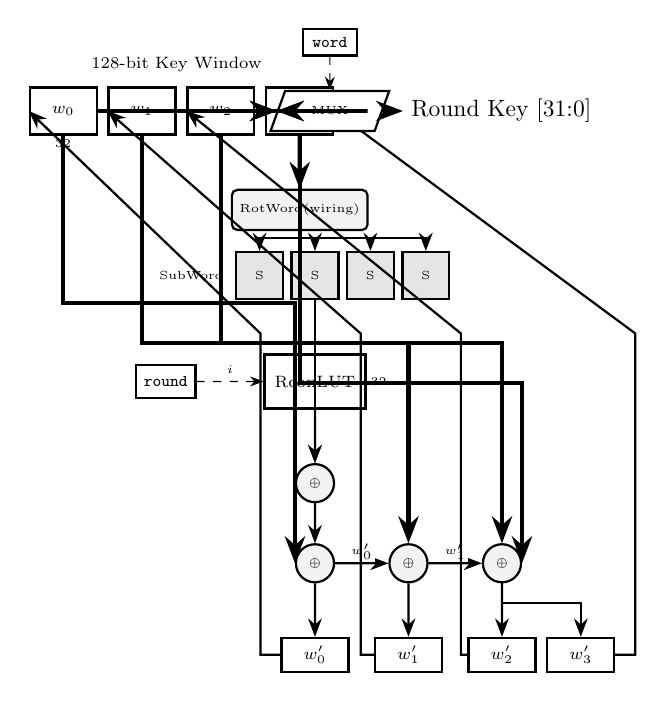
\begin{tikzpicture}[node distance=0.6cm and 0.8cm, scale=0.85, transform shape]

% Current key window registers
\node[register, minimum width=1cm, minimum height=0.7cm] (w0) {$w_0$};
\node[register, minimum width=1cm, minimum height=0.7cm, right=0.15cm of w0] (w1) {$w_1$};
\node[register, minimum width=1cm, minimum height=0.7cm, right=0.15cm of w1] (w2) {$w_2$};
\node[register, minimum width=1cm, minimum height=0.7cm, right=0.15cm of w2] (w3) {$w_3$};

\node[font=\scriptsize, above=0.1cm of w1.north east] {128-bit Key Window};
\node[buswidth] at (w0.south) [below=0.02cm] {32};

% RotWord - just wiring
\node[logic, below=0.8cm of w3, minimum width=1cm] (rotword) {RotWord\\(wiring)};
\draw[bus] (w3) -- (rotword);

% S-box array
\node[sbox, below=0.3cm of rotword, xshift=-0.6cm] (ks0) {S};
\node[sbox, right=0.1cm of ks0] (ks1) {S};
\node[sbox, right=0.1cm of ks1] (ks2) {S};
\node[sbox, right=0.1cm of ks2] (ks3) {S};

\draw[wire] (rotword.south) -- ++(0,-0.1) -| (ks0.north);
\draw[wire] (rotword.south) -- ++(0,-0.1) -| (ks1.north);
\draw[wire] (rotword.south) -- ++(0,-0.1) -| (ks2.north);
\draw[wire] (rotword.south) -- ++(0,-0.1) -| (ks3.north);

\node[font=\tiny, left=0.05cm of ks0.west] {SubWord};

% Rcon LUT
\node[memory, below=0.8cm of ks1, minimum width=1.5cm, minimum height=0.8cm] (rcon) {Rcon\\LUT};
\node[buswidth] at (rcon.east) [right=0.02cm] {32};

% XOR operations
\node[logic, circle, minimum size=0.4cm, below=0.8cm of rcon] (xor1) {$\oplus$};
\node[logic, circle, minimum size=0.4cm, below=0.6cm of xor1] (xor2) {$\oplus$};
\node[logic, circle, minimum size=0.4cm, right=0.8cm of xor2] (xor3) {$\oplus$};
\node[logic, circle, minimum size=0.4cm, right=0.8cm of xor3] (xor4) {$\oplus$};

% Connect S-boxes to first XOR
\draw[wire] (ks1.south) -- ++(0,-0.2) -| (xor1.north);

% Connect Rcon
\draw[wire] (rcon) -- (xor1);

% Connect w0 to XOR chain
\draw[bus] (w0.south) -- ++(0,-2.5) -| (xor2.west);

% XOR chain
\draw[wire] (xor1) -- (xor2);
\draw[wire] (xor2) -- node[buswidth, above] {$w_0'$} (xor3);

% w1, w2, w3 to XOR chain
\draw[bus] (w1.south) -- ++(0,-3.1) -| (xor3.north);
\draw[bus] (w2.south) -- ++(0,-3.1) -| (xor4.north);

\draw[wire] (xor3) -- node[buswidth, above] {$w_1'$} (xor4);

% Output and feedback
\node[register, below=0.8cm of xor2, minimum width=1cm, minimum height=0.5cm] (w0_new) {$w_0'$};
\node[register, below=0.8cm of xor3, minimum width=1cm, minimum height=0.5cm] (w1_new) {$w_1'$};
\node[register, below=0.8cm of xor4, minimum width=1cm, minimum height=0.5cm] (w2_new) {$w_2'$};

\draw[wire] (xor2) -- (w0_new);
\draw[wire] (xor3) -- (w1_new);
\draw[wire] (xor4) -- (w2_new);

% w3 direct connection
\draw[bus] (w3.south) -- ++(0,-3.7) -| (xor4.east);
\node[register, right=0.15cm of w2_new, minimum width=1cm, minimum height=0.5cm] (w3_new) {$w_3'$};
\draw[wire] (xor4.south) -- ++(0,-0.3) -| (w3_new.north);

% Feedback to registers
\draw[wire] (w0_new.west) -- ++(-0.3,0) -- ++(0,4.8) -- (w0.west);
\draw[wire] (w1_new.west) -- ++(-0.2,0) -- ++(0,4.8) -- (w1.west);
\draw[wire] (w2_new.west) -- ++(-0.1,0) -- ++(0,4.8) -- (w2.west);
\draw[wire] (w3_new.east) -- ++(0.3,0) -- ++(0,4.8) -- (w3.east);

% Round counter
\node[register, left=1cm of rcon, minimum width=0.8cm, minimum height=0.5cm] (round) {round};
\draw[controlwire] (round) -- node[above, font=\tiny] {$i$} (rcon);

% Output mux
\node[mux, right=1.5cm of w1, minimum width=1cm] (outmux) {MUX};
\draw[bus] (w0.east) -- ++(0.2,0) |- (outmux.west);
\draw[bus] (w1.east) -- ++(0.3,0) |- (outmux.west);
\draw[bus] (w2.east) -- ++(0.4,0) |- (outmux.west);
\draw[bus] (w3.east) -- ++(0.5,0) |- (outmux.west);

\node[right=0.3cm of outmux] (keyout) {Round Key [31:0]};
\draw[bus] (outmux) -- (keyout);

% Control
\node[register, above=0.5cm of outmux, minimum width=0.8cm, minimum height=0.4cm] (word_cnt) {word};
\draw[controlwire] (word_cnt) -- (outmux);

\end{tikzpicture}
\caption{On-the-fly key expansion hardware. Only four 32-bit word registers ($w_0$--$w_3$) are stored, updated each round using SubWord, RotWord, and Rcon operations. This achieves 90\% memory reduction versus storing all 44 words.}
\label{fig:key_hardware}
\end{figure}

%==============================================================================
% Figure 4: SubBytes S-box Implementation
%==============================================================================
\begin{figure}[t]
\centering
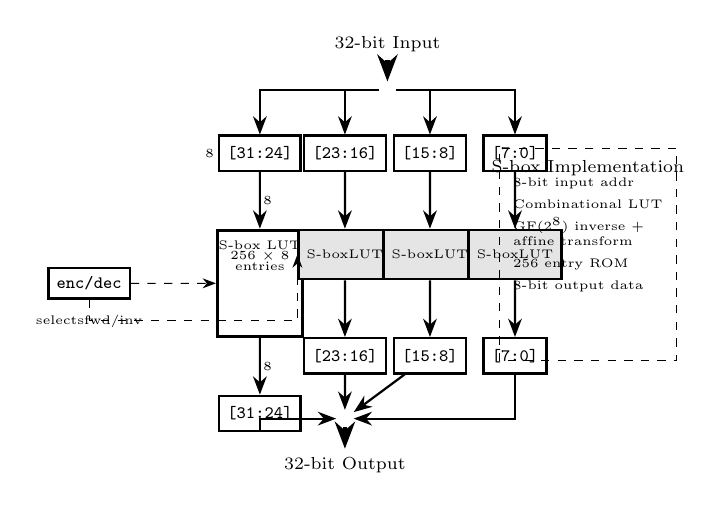
\begin{tikzpicture}[node distance=0.6cm and 0.8cm, scale=0.9, transform shape]

% 32-bit input
\node[font=\scriptsize] (input) {32-bit Input};
\node[below=0.3cm of input] (bus_split) {};

% Split into bytes
\node[register, below=0.5cm of bus_split, xshift=-1.8cm, minimum width=0.8cm, minimum height=0.5cm] (b0) {[31:24]};
\node[register, below=0.5cm of bus_split, xshift=-0.6cm, minimum width=0.8cm, minimum height=0.5cm] (b1) {[23:16]};
\node[register, below=0.5cm of bus_split, xshift=0.6cm, minimum width=0.8cm, minimum height=0.5cm] (b2) {[15:8]};
\node[register, below=0.5cm of bus_split, xshift=1.8cm, minimum width=0.8cm, minimum height=0.5cm] (b3) {[7:0]};

\draw[bus] (input) -- (bus_split);
\draw[wire] (bus_split) -| (b0);
\draw[wire] (bus_split) -| (b1);
\draw[wire] (bus_split) -| (b2);
\draw[wire] (bus_split) -| (b3);

\node[buswidth] at (b0.west) [left=0.02cm] {8};

% S-box LUT (detailed for one)
\node[memory, below=0.8cm of b0, minimum width=1.2cm, minimum height=1.5cm] (sbox0) {};
\node[font=\tiny, below=0.05cm of sbox0.north] {S-box LUT};
\node[font=\tiny, below=0.2cm of sbox0.north] {256 $\times$ 8};
\node[font=\tiny, below=0.35cm of sbox0.north] {entries};

% Other S-boxes (simplified)
\node[sbox, below=0.8cm of b1] (sbox1) {S-box\\LUT};
\node[sbox, below=0.8cm of b2] (sbox2) {S-box\\LUT};
\node[sbox, below=0.8cm of b3] (sbox3) {S-box\\LUT};

% Connections to S-boxes
\draw[wire] (b0) -- node[buswidth, right] {8} (sbox0);
\draw[wire] (b1) -- (sbox1);
\draw[wire] (b2) -- (sbox2);
\draw[wire] (b3) -- (sbox3);

% Output bytes
\node[register, below=0.8cm of sbox0, minimum width=0.8cm, minimum height=0.5cm] (ob0) {[31:24]};
\node[register, below=0.8cm of sbox1, minimum width=0.8cm, minimum height=0.5cm] (ob1) {[23:16]};
\node[register, below=0.8cm of sbox2, minimum width=0.8cm, minimum height=0.5cm] (ob2) {[15:8]};
\node[register, below=0.8cm of sbox3, minimum width=0.8cm, minimum height=0.5cm] (ob3) {[7:0]};

\draw[wire] (sbox0) -- node[buswidth, right] {8} (ob0);
\draw[wire] (sbox1) -- (ob1);
\draw[wire] (sbox2) -- (ob2);
\draw[wire] (sbox3) -- (ob3);

% Merge
\node[below=0.5cm of ob1] (bus_merge) {};
\node[font=\scriptsize, below=0.3cm of bus_merge] (output) {32-bit Output};

\draw[wire] (ob0) |- (bus_merge);
\draw[wire] (ob1) -- (bus_merge);
\draw[wire] (ob2) -- (bus_merge);
\draw[wire] (ob3) |- (bus_merge);
\draw[bus] (bus_merge) -- (output);

% S-box detail
\node[draw, dashed, right=1.5cm of sbox1, minimum width=2.5cm, minimum height=3cm] (sbox_detail) {};
\node[font=\scriptsize, below=0.05cm of sbox_detail.north] {S-box Implementation};

\node[font=\tiny, below=0.3cm of sbox_detail.north, align=left] {
8-bit input addr\\[0.1cm]
Combinational LUT\\[0.1cm]
$\text{GF}(2^8)$ inverse + \\
affine transform\\[0.1cm]
256 entry ROM\\[0.1cm]
8-bit output data
};

% Control
\node[register, left=1.2cm of sbox0, minimum width=0.8cm, minimum height=0.4cm] (mode) {enc/\\dec};
\draw[controlwire] (mode) -- (sbox0.west);
\draw[controlwire] (mode.south) -- ++(0,-0.3) -| (sbox1.west);

\node[font=\tiny, below=0.1cm of mode] {selects\\fwd/inv};

\end{tikzpicture}
\caption{SubBytes hardware with four parallel S-box lookup tables. Each S-box is a 256$\times$8-bit combinational ROM implementing the AES substitution. The enc/dec control selects forward or inverse S-box.}
\label{fig:subbytes_hw}
\end{figure}

%==============================================================================
% Figure 5: MixColumns Hardware
%==============================================================================
\begin{figure}[t]
\centering
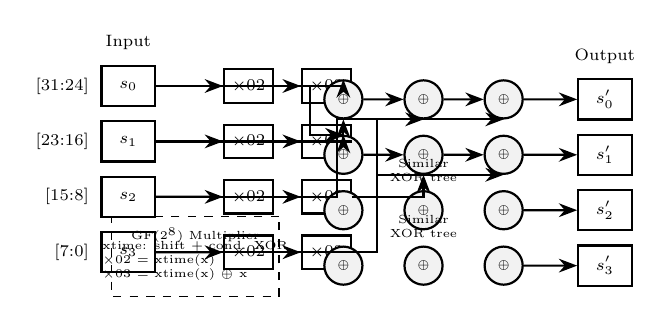
\begin{tikzpicture}[node distance=0.5cm and 0.6cm, scale=0.85, transform shape]

% Input column
\node[register, minimum width=0.8cm, minimum height=0.6cm] (s0) {$s_0$};
\node[register, minimum width=0.8cm, minimum height=0.6cm, below=0.2cm of s0] (s1) {$s_1$};
\node[register, minimum width=0.8cm, minimum height=0.6cm, below=0.2cm of s1] (s2) {$s_2$};
\node[register, minimum width=0.8cm, minimum height=0.6cm, below=0.2cm of s2] (s3) {$s_3$};

\node[font=\scriptsize, above=0.1cm of s0] {Input};
\node[font=\scriptsize, left=0.05cm of s0.west] {[31:24]};
\node[font=\scriptsize, left=0.05cm of s1.west] {[23:16]};
\node[font=\scriptsize, left=0.05cm of s2.west] {[15:8]};
\node[font=\scriptsize, left=0.05cm of s3.west] {[7:0]};

% GF multipliers for s0
\node[alu, right=1cm of s0, minimum width=0.7cm, minimum height=0.5cm] (m02_0) {$\times$02};
\node[alu, right=0.4cm of m02_0, minimum width=0.7cm, minimum height=0.5cm] (m03_0) {$\times$03};

% GF multipliers for s1
\node[alu, right=1cm of s1, minimum width=0.7cm, minimum height=0.5cm] (m02_1) {$\times$02};
\node[alu, right=0.4cm of m02_1, minimum width=0.7cm, minimum height=0.5cm] (m03_1) {$\times$03};

% GF multipliers for s2
\node[alu, right=1cm of s2, minimum width=0.7cm, minimum height=0.5cm] (m02_2) {$\times$02};
\node[alu, right=0.4cm of m02_2, minimum width=0.7cm, minimum height=0.5cm] (m03_2) {$\times$03};

% GF multipliers for s3
\node[alu, right=1cm of s3, minimum width=0.7cm, minimum height=0.5cm] (m02_3) {$\times$02};
\node[alu, right=0.4cm of m02_3, minimum width=0.7cm, minimum height=0.5cm] (m03_3) {$\times$03};

% Connections to multipliers
\draw[wire] (s0) -- (m02_0);
\draw[wire] (s0.east) -- ++(0.3,0) |- (m03_0.west);
\draw[wire] (s1) -- (m02_1);
\draw[wire] (s1.east) -- ++(0.3,0) |- (m03_1.west);
\draw[wire] (s2) -- (m02_2);
\draw[wire] (s2.east) -- ++(0.3,0) |- (m03_2.west);
\draw[wire] (s3) -- (m02_3);
\draw[wire] (s3.east) -- ++(0.3,0) |- (m03_3.west);

% XOR trees for output
\node[logic, circle, minimum size=0.35cm, right=2.5cm of s0, yshift=-0.2cm] (xor0_1) {$\oplus$};
\node[logic, circle, minimum size=0.35cm, right=0.6cm of xor0_1] (xor0_2) {$\oplus$};
\node[logic, circle, minimum size=0.35cm, right=0.6cm of xor0_2] (xor0_3) {$\oplus$};

\node[logic, circle, minimum size=0.35cm, right=2.5cm of s1, yshift=-0.2cm] (xor1_1) {$\oplus$};
\node[logic, circle, minimum size=0.35cm, right=0.6cm of xor1_1] (xor1_2) {$\oplus$};
\node[logic, circle, minimum size=0.35cm, right=0.6cm of xor1_2] (xor1_3) {$\oplus$};

\node[logic, circle, minimum size=0.35cm, right=2.5cm of s2, yshift=-0.2cm] (xor2_1) {$\oplus$};
\node[logic, circle, minimum size=0.35cm, right=0.6cm of xor2_1] (xor2_2) {$\oplus$};
\node[logic, circle, minimum size=0.35cm, right=0.6cm of xor2_2] (xor2_3) {$\oplus$};

\node[logic, circle, minimum size=0.35cm, right=2.5cm of s3, yshift=-0.2cm] (xor3_1) {$\oplus$};
\node[logic, circle, minimum size=0.35cm, right=0.6cm of xor3_1] (xor3_2) {$\oplus$};
\node[logic, circle, minimum size=0.35cm, right=0.6cm of xor3_2] (xor3_3) {$\oplus$};

% Output row 0: 02*s0 ⊕ 03*s1 ⊕ s2 ⊕ s3
\draw[wire] (m02_0) -| (xor0_1);
\draw[wire] (m03_1) -| (xor0_1);
\draw[wire] (xor0_1) -- (xor0_2);
\draw[wire] (s2.east) -- ++(2.7,0) |- (xor0_2.south);
\draw[wire] (xor0_2) -- (xor0_3);
\draw[wire] (s3.east) -- ++(3.3,0) |- (xor0_3.south);

% Output row 1: s0 ⊕ 02*s1 ⊕ 03*s2 ⊕ s3
\draw[wire] (s0.east) -- ++(2.3,0) |- (xor1_1.north);
\draw[wire] (m02_1) -| (xor1_1);
\draw[wire] (xor1_1) -- (xor1_2);
\draw[wire] (m03_2) -| (xor1_2);
\draw[wire] (xor1_2) -- (xor1_3);
\draw[wire] (s3.east) -- ++(3.3,0) |- (xor1_3.south);

% Output registers
\node[register, right=0.8cm of xor0_3, minimum width=0.8cm, minimum height=0.6cm] (out0) {$s_0'$};
\node[register, right=0.8cm of xor1_3, minimum width=0.8cm, minimum height=0.6cm] (out1) {$s_1'$};
\node[register, right=0.8cm of xor2_3, minimum width=0.8cm, minimum height=0.6cm] (out2) {$s_2'$};
\node[register, right=0.8cm of xor3_3, minimum width=0.8cm, minimum height=0.6cm] (out3) {$s_3'$};

\draw[wire] (xor0_3) -- (out0);
\draw[wire] (xor1_3) -- (out1);
\draw[wire] (xor2_3) -- (out2);
\draw[wire] (xor3_3) -- (out3);

\node[font=\scriptsize, above=0.1cm of out0] {Output};

% Simplified for s2 and s3
\node[font=\tiny] at (xor2_2) [above=0.3cm, align=center] {Similar\\XOR tree};
\node[font=\tiny] at (xor3_2) [above=0.3cm, align=center] {Similar\\XOR tree};

% GF multiplier detail
\node[draw, dashed, below=0.8cm of s1, minimum width=2.5cm, minimum height=1.2cm, xshift=1cm] (gf_detail) {};
\node[font=\tiny, below=0.05cm of gf_detail.north] {GF($2^8$) Multiplier};
\node[font=\tiny, below=0.25cm of gf_detail.north, align=left] {
xtime: shift + cond. XOR\\
$\times$02 = xtime(x)\\
$\times$03 = xtime(x) $\oplus$ x
};

\end{tikzpicture}
\caption{MixColumns hardware implementing matrix multiplication in GF($2^8$). Each output byte uses dedicated GF multipliers ($\times$02, $\times$03) and XOR trees. The $\times$02 operation (xtime) is a shift with conditional XOR by 0x1B.}
\label{fig:mixcol_hw}
\end{figure}

%==============================================================================
% Figure 6: Control FSM Hardware
%==============================================================================
\begin{figure}[t]
\centering
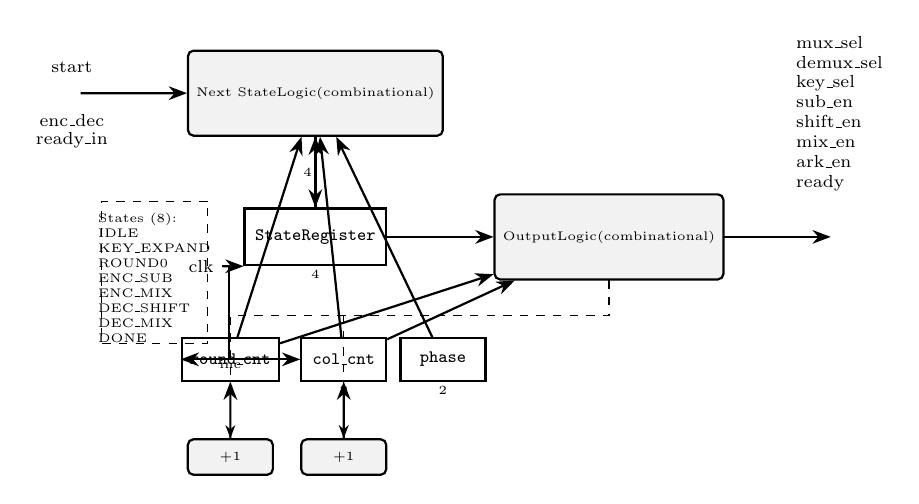
\begin{tikzpicture}[node distance=0.7cm and 1cm, scale=0.9, transform shape]

% State register
\node[register, minimum width=2cm, minimum height=0.8cm] (state_reg) {State\\Register};
\node[buswidth] at (state_reg.south) [below=0.02cm] {4};

% Next state logic
\node[logic, above=1cm of state_reg, minimum width=2.5cm, minimum height=1.2cm] (nsl) {Next State\\Logic\\(combinational)};

% Output logic
\node[logic, right=1.5cm of state_reg, minimum width=2.5cm, minimum height=1.2cm] (output_logic) {Output\\Logic\\(combinational)};

% Counters
\node[register, below=1cm of state_reg, xshift=-1.2cm, minimum width=1.2cm, minimum height=0.6cm] (round_cnt) {round\_cnt};
\node[buswidth] at (round_cnt.south) [below=0.02cm] {4};

\node[register, below=1cm of state_reg, xshift=0.4cm, minimum width=1.2cm, minimum height=0.6cm] (col_cnt) {col\_cnt};
\node[buswidth] at (col_cnt.south) [below=0.02cm] {2};

\node[register, below=1cm of state_reg, xshift=1.8cm, minimum width=1.2cm, minimum height=0.6cm] (phase) {phase};
\node[buswidth] at (phase.south) [below=0.02cm] {2};

% Counter logic
\node[logic, below=0.8cm of round_cnt, minimum width=1.2cm, minimum height=0.5cm] (round_inc) {+1};
\node[logic, below=0.8cm of col_cnt, minimum width=1.2cm, minimum height=0.5cm] (col_inc) {+1};

% Inputs
\node[left=1.5cm of nsl] (inputs) {};
\node[font=\scriptsize, above=0.05cm of inputs] {start};
\node[font=\scriptsize, below=0.05cm of inputs] {enc\_dec};
\node[font=\scriptsize, below=0.3cm of inputs] {ready\_in};

% Outputs
\node[right=1.5cm of output_logic] (outputs) {};
\node[font=\scriptsize, above=0.4cm of outputs, align=left] {
mux\_sel\\
demux\_sel\\
key\_sel\\
sub\_en\\
shift\_en\\
mix\_en\\
ark\_en\\
ready
};

% Control flow
\draw[wire] (state_reg) -- (nsl);
\draw[wire] (nsl) -- node[buswidth, left] {4} (state_reg);
\draw[wire] (state_reg) -- (output_logic);
\draw[wire] (output_logic) -- (outputs);
\draw[wire] (inputs) -- (nsl);

% Counter connections
\draw[wire] (round_cnt) -- (nsl);
\draw[wire] (col_cnt) -- (nsl);
\draw[wire] (phase) -- (nsl);

\draw[wire] (round_cnt) -- (output_logic);
\draw[wire] (col_cnt) -- (output_logic);

\draw[controlwire] (output_logic.south) -- ++(0,-0.5) -| node[near end, above, font=\tiny] {inc} (round_inc.north);
\draw[controlwire] (output_logic.south) -- ++(0,-0.5) -| (col_inc.north);

\draw[wire] (round_inc) -- (round_cnt);
\draw[wire] (col_inc) -- (col_cnt);

% Clock
\node[left=0.3cm of state_reg.south west] (clk) {\scriptsize clk};
\draw[wire] (clk) -- (state_reg.south west);
\draw[wire] (clk.east) -- ++(0.1,0) |- (round_cnt.west);
\draw[wire] (clk.east) -- ++(0.1,0) |- (col_cnt.west);

% States annotation
\node[draw, dashed, left=0.5cm of state_reg, minimum width=1.5cm, minimum height=2cm, yshift=-0.5cm] (states) {};
\node[font=\tiny, below=0.05cm of states.north, align=left] {
States (8):\\
IDLE\\
KEY\_EXPAND\\
ROUND0\\
ENC\_SUB\\
ENC\_MIX\\
DEC\_SHIFT\\
DEC\_MIX\\
DONE
};

\end{tikzpicture}
\caption{Control FSM hardware showing state register, next-state logic, output logic, and round/column counters. All control signals are generated combinationally from current state and counter values.}
\label{fig:control_fsm}
\end{figure}

\end{document}
